\chapter{Scientific Programming}
\label{ch:SciProg}

The introduction of the computer around World War II had a major impact on the mathematical fields of science. Previously unsolvable problems were now  solvable. The question was no longer whether or not it was possible, but rather to what precision and with which method. The computer spawned a new branch of physics, \textit{computational physics}, breaching barriers no one could even imagine existed. The first major result of this synergy between science and computers came with the infamous atomic bombs \textit{Little Boy} and \textit{Fat Man}, a product of \textit{The Manhattan Project} leaded by \textit{J. Robert Oppenheimer} \cite{supermen}.

\section{Programming Languages}

Writing a program, or a code, is a list of instructions for the computer. It is in many ways similar to writing human-to-human instructions. You may use different programming languages, such as C++, Python, Java, as long as the reader is able to translate it. The translator, called \textit{compiler} or \textit{interpreter}, translates your program from e.g. C++ code to machine code. Other languages such as Python are interpreted real-time and therefore require no compilation; it instructs as it reads. Although the latter seems like a better solution, it comes at the price of efficiency, a key concept in programming. 

As a rule of thumb, efficiency is inverse proportional to the complexity of the programming language. It is therefore natural to sort languages into different subgroups depending on where they are at the efficiency-complexity scale.


\subsection{High-level Languages}

Scientific programming is more than number crunching loops. This section's subgroup of languages are often referred to as \textit{scripting languages}. A script is a short code with a specific aim such as analyzing raw data, administrating input and output from different tools, creating a \textit{Graphical User Interface} (GUI), or gluing together different programs which are meant to be run sequentially or in parallel \cite{inf3331}.

For these types of jobs, the relief of simple rigorous syntax weighs up for the efficiency penalty. In most cases, the runtime of the program is so small that efficiency becomes irrelevant, leaving scripting languages the optimal tool for the task. These languages which prefer simplicity over efficiency are referred to as \textit{High-level} \footnote{There are different definitions of high-level vs. low-level. You have languages such as \textit{assembly}, which is extremely complex and close to machine code, leaving all machine-independent languages as high-level ones. However, for the purpose of this thesis I will not go into assembly languages, and keep the distinction at a higher level.}. Examples of high-level languages are Python, Ruby, Perl, Visual Basic and UNIX shells. In this thesis, Python is the mainly used scripting language.   

\subsubsection{Python}
\label{sec:Python}

Python is a programming language with a focus on being simple to learn and have a very clean syntax \cite{inf1100, inf3331}. To mention a few of the entries in the \textit{Zen of Python}\footnote{Retrieved by typing ``import this'' in your Python shell.}, ``Beautiful is better than ugly. Simple is better than complex. Readability counts. If the implementation is hard to explain, it's a bad idea.''

To demonstrate the simplicity of Python, let us have a look at a simple implementation and execution of the following expression

\[
 S = \sum_{i=1}^{100} i = 5050.  \label{eq:sum100}
\]

\lstinputlisting[language=Python]{../CodeInputs/Sum100Python.py}


\begin{verbatim}
~$ python Sum100Python.py 
5050
\end{verbatim}




\subsection{Low-level Languages}
\label{sec:lowlevel}

A huge part of scientific programming involves solving complex equations. Complexity does not necessarily imply that the equations themselves are hard to understand; frankly, this is often not the case. In most cases of e.g. linear algebra, the problem can be boiled down to solving $A\vec x = B$, however, the complexity lies in the dimensionality of the problem at hand. Matrix dimensions range as high as millions. With each element being a double precision number (8 bytes or 64 bits), it is crucial that we have full control of the memory, and execute operations as efficiently as possible. 

This is where lower level languages excel. Hiding few to none of the details, the power is in the hand of the programmer. This comes at a price: More technical concepts such as memory pointers, declarations, compiling, linking, etc. makes the development process slower than that of a higher-level language. If you e.g. try to access an element outside the bounds of an array, Python would tell you a detailed error message with proper traceback, whereas the compiled C++ code would crash runtime leaving nothing but a ``segmentation fault'' for the user. However, when the optimized program ends up running for days, the extra time spent in development pays off. In addition you have several options to optimize your compiled machine code by having the compiler rearrange the way instructions are sent to the processor\footnote{I will not go more into details on this topic. For more information research topics such as \textit{CPU cache}, \textit{Memory bus latency} and \textit{CPU architecture} in general.} (without 
ruining it of course), which interpreted languages does not have. 

\subsubsection{C++}

C++ is a programming language developed by Bjarne Stroustrup in 1983. It serves as an extension to the original \textit{C} language, adding object oriented features, that is, classes etc. \cite{ORegan}. The following code is a C++ implementation of the sum in Eq.~\ref{eq:sum100}:

\vspace{0.5 cm}
\lstinputlisting[language=c++]{../CodeInputs/Sum100C++.cpp}

\begin{verbatim}
~$ g++ Sum100C++.cpp -o sum100C++.x
~$ ./sum100C++.x 
5050
\end{verbatim}


As we can see in lines five and six, we need to declare \textit{S} and \textit{i} as integer variables, exactly as described in section~\ref{sec:lowlevel}. In comparison with the Python version, it is clear that lower level languages are more complicated, and not designed for simple jobs as calculating a single sum.

Even though this is an extremely simply example, it illustrates the difference in coding styles between high- and low-level languages: Complexity vs. simplicity, efficiency vs. readability. I will not go through all the basic details of C++, but rather focus on the more complicated parts involving object orientation in scientific programming.


\section{Object Orientation}
\label{sec:OO}

Object orientated programming was introduced in the language \textit{Simula 67}, developed by the Norwegian scientists Ole-Johan Dahl and Kristen Nygaard at the Norwegian Computing Research Center \cite{ORegan}. It quickly became the state-of-the-art in programming, and is today used throughout the world in all branches of programming. It is brilliant in the way that it ties our everyday intuition into the programming language - our brain is object oriented. It is focused around the concept of \textit{classes}, a collection of variables and functions aimed for a specific task. In a program, instances of classes, or \textit{objects}, are created and can be viewed as independent actors aimed for specific tasks \cite{inf1100, inf3331, ORegan}. However, they provide a great deal of functionality like e.g. \textit{inheritance} and accessibility control. 

\subsection{Inheritance}

Consider the abstract idea of a keyboard. All keyboards have two things in common: A board and keys (obviously). In object orientation we would say that the \textit{superclass} of keyboards describe a board with keys. It is \textit{abstract} in the sense that you do not need to know what the keys look like, or what function they possess, in order to define the concept of a keyboard.

However, we can have different types of keyboards, for example a computer keyboard, or a musical keyboard. They are different in design and function, but they both relate to the same concept of a keyboard described previously. They are both \textit{subclasses} of the same superclass, inheriting the basic concepts, but expands upon them defining their own specific case. 

I will present examples assuming the reader is somewhat familiar to programming concepts and basic Python. On the following page an example implementation of a Keyboard class in Python is listed.

\newpage
\lstinputlisting[language=Python]{../CodeInputs/KeyboardClassPython.py}

As we can see, the only thing differentiating the two keyboard types are how the keys are set up, and what happens when we press one of them. A superclass function designed to be overridden is referred to as \textit{virtual}. If the function is not even implemented, they are referred to as \textit{pure virtual} in the sense that they should be overwritten by any subclass. More on this in the next section.

\subsection{Pointers, Virtual Functions and Types}

A pointer is a hexadecimal number representing a memory address where some \textit{type} of object is stored, e.g. a \verb+int+ at \verb+0x7fff0882306c+. Higher level languages like Python handles all the pointers and typesetting by themselves. In low-level languages like C++, however, you need to control everything. If you pass a pointer to an object, e.g. \verb+Keyboard* myKeyboard+, as an argument to a function, whenever that function makes changes to the object, the object is changed globally, since the memory address is directly accessed. If you instead choose to send the object without a pointer declaration, e.g. \verb+Keyboard myKeyboard+, changing the value will not change the object globally. What happens instead is that you change a local copy of the object. However, once you crack the code, pointers are dear friends, not lethal enemies.

Virtual functions are functions designed for overriding; \verb+virtual+ is a flag telling the compiler to search for the deepest implementation of the specific function (in terms of subclassing) no matter the original type. \verb+setupKeys+ and \verb+pressKey+ are examples of this, however, they are in a sense more than virtual, since they are not even implemented, namely pure virtual; they have to be overridden in order to work. 

In python, we never come into trouble with virtual functions, since you don't manually control the object type. In C++ however, we have to specify whether or not a function is virtual in the declaration in order to achieve the desired functionality. This because an instance of \verb+ComputerKeyboard+ could either be of type \verb+ComputerKeyboard+ or \verb+Keyboard+. The next example will illustrate this. 

\vspace{0.5 cm}
\lstinputlisting[language=c++]{../CodeInputs/virtualFunctionsC++.cpp}

\begin{verbatim}
~$ ./virtualFunctionsC++.x 
-Calling subClass object of type superClass*
subclass pure virtual override
subclass standard virtual override
superclass notVirtual

-Calling subClass object of type subClass*
subclass pure virtual override
subclass standard virtual override
superclass notVirtual

-Directly calling object of type subclass*
subclass pure virtual override
subclass standard virtual override
subclass non virtual
\end{verbatim}

\subsection*{Typecasting and Polymorphism}
\label{sec:typeCastPoly}

In order to understand these concepts, consider the previous example. In the first call, the object is declared as a \verb+superClass*+ type, however, it is still initialized to be a \verb+subClass+ pointer, which results in the subclass' functions overriding the corresponding ones of the superclass, given they are virtual. In programming terms we say that \textit{any subclass is type-compatible with a pointer to it's superclass}.%[cite http://www.cplusplus.com/doc/tutorial/polymorphism/]. 

In the second call, the same thing happens, even though it is set as a \verb+subclass*+ type. This is because the function is instructed to receive a \verb+superClass*+ input. If it receives anything else, it simply attempts to convert it, or \textit{cast} it, to the specified type; \textit{typecasting}\footnote{The standard example of typecasting is converting a double to an integer, resulting in the stripping of all the decimal bits (flooring).}. As discussed in the previous paragraph casting from a subclass to its superclass is allowed. The third call, outside the function, demonstrates that if we do not typecast the object, the object's functions consists solely of its own, virtual or not.

This all boils down to one powerful concept in object orientated programming, namely \textit{polymorphism}. Polymorphism is the scenario where e.g. a function is declared to receive a superclass pointer (like \verb+testFunc+), yet when it's called, it's called with subclass implementations of the superclass (the second call described above). The function is instructed to call member functions of the subclass, however, we can override these by declaring them as virtual functions. In other words, the code can be written extremely organized and versatile given proper use of polymorphism. To further illustrate this, consider the following example from the Quantum Monte Carlo code developed in this thesis, more spesificly 

\vspace{0.5 cm}
\begin{lstlisting}
class Potential {
protected:
    int n_p;
    int dim;

public:
    Potential(int n_p, int dim);
    Potential();

    virtual double get_pot_E(const Walker* walker) const = 0;

};

class Coulomb : public Potential {
public:

    Coulomb(GeneralParams &);

    virtual double get_pot_E(const Walker* walker) const;

};

class Harmonic_osc : public Potential {
protected:
    double w;

public:

    Harmonic_osc(GeneralParams &);

    double get_pot_E(const Walker* walker) const;

};

\end{lstlisting}
\begin{lstlisting}
double Coulomb::get_pot_E(const Walker* walker) const {

    double e_coulomb = 0;

    for (int i = 0; i < n_p - 1; i++) {
        for (int j = i + 1; j < n_p; j++) {
            e_coulomb += 1 / walker->r_rel(i,j);
        }
    }

    return e_coulomb;
}

double Harmonic_osc::get_pot_E(const Walker* walker) const {

    double e_potential = 0;

    for (int i = 0; i < n_p; i++) {
        e_potential += 0.5 * w * w * walker->get_r_i2(i);
    }

    return e_potential;
}
\end{lstlisting}


This subclass hierarchy of potentials instructs the system to access objects of type \verb+Potential*+, calling the objects function \verb+get_pot_E+ with the current walker as input. Or, even more powerfully, we can assign any number of \verb+Potential*+ objects to the system, and simply iterate through them and accumulate their energy contributions:

\vspace{0.5cm}
\begin{lstlisting}
class System {
protected:
    ...
    
    std::vector<Potential*> potentials;
    
    ...
};

double System::get_potential_energy(const Walker* walker) {
    double potE = 0;

    //Iterate through the potential objects in the potentials list. (*pot) extracts the pointer from the iterator.
    for (std::vector<Potential*>::iterator pot = potentials.begin(); pot != potentials.end(); ++pot) {
        potE += (*pot)->get_pot_E(walker);
    }

    return potE;
}
\end{lstlisting}


The objects in the list can be any subclass implementation of the \verb+Potential+ class, all the compiler needs to know is that it has a method \verb+get_pot_E+ that it can call on runtime. Polymorphism creates a port for versatile code structures. It does not matter whether seven different potentials are loaded or none at all. Versatile, generalized, yet beautiful. 

\subsection{Const Correctness}

In the \verb+Potential+ code example above, function declarations with \verb+const+ are used. If an object is declared with \verb+const+ on input, e.g. \verb+void f(const x)+, the function itself cannot alter the value of \verb+x+. It is a safeguard that nothing will happen to \verb+x+ as it passes through \verb+f+. This is practical in situations where major bugs will arise if anything happens to an object, yet you do not want to copy it on input.

If you declare a member function itself with \verb+const+ on the right hand side, it safeguards the function from changing any of the class variables. If you e.g. have a variable representing the electron charge, you do not want this changed by the Coulomb class member function. This should only happen through specific functions whose sole purpose is changing the charge, and taking care of any following consequences. 

In other words: \verb+const+ works as a safeguard for changing values which should remain unchanged. A change in such a variable is then followed by a compiler error instead of infecting your code with bugs, resulting in unforeseen consequences.

\subsection{Accessibility levels and Friend classes}

\verb+const+ is a direct way to avoid any change what so ever. However, sometimes we want to keep the ability to alter variables, but only in certain situations, as e.g. internally in the class. As an example, from the main file, you should not have access to \verb+QMC+ member functions such as \verb+dump_output+, since it does not make sense, or is directly dangerous, to do out of a context. However, you obviously want access to the \verb+run_method+ function.

The solution to this problem is to set accessibility levels. Declaring a variable under the \verb+public+ part of a class sets its accessibility level to \textit{public}, meaning that anything, anywhere can access it as long as it has access to the object. Declarations beneath the \verb+private+ part stops all other classes than instances of itself from reaching it, even subclass instances. If you want private variables inherited, the \verb+protected+ accessibility level should be used, this ensures that the members are hidden for everyone except the class itself and its subclasses.

There is one exception to the rule of protected and private variables, namely \textit{friend} classes. In the QMC code, there is a output class called \verb+OutputHandler+. This class needs access to protected variables, since the user should be able to output anything he wants. If we \verb+friend+ the output class with \verb+QMC+, we get exactly this behavior: 

\vspace{0.5 cm}
\begin{lstlisting}[language=c++]

class QMC {
protected:
    
    ...
    
    std::stringstream s; 
    
    ...
    
    int n_c;

    ...

    int cycle;

    ...

public:

    ...

};

class VMC : public QMC {
protected:

    ...

    Walker* original_walker;
    Walker* trial_walker;

    ...

public:

    ...

    friend class Distribution;
    ...

};
\end{lstlisting}

\begin{lstlisting}[language=c++]
void Distribution::dump() {

    //if we are more than half way we save a snapshot of the walker every 100'th step
    if ((vmc->cycle >= vmc->n_c / 2) && (vmc->cycle % 100 == 0)) {
        
        //s: unique file name for the current snapshot of the diffusing walker
        s << path << "walker_positions/" << filename << node <<"_"<< i <<".arma";
        
        //saves the position matrix to file
        vmc->original_walker->r.save(s.str());
        
        //clears the stringstream and iterates identifyer 'i'
        s.str(std::string());
        i++;
    }
}
\end{lstlisting}

Without going into details, we can see that \verb+Distribution+ has full access to protected, or hidden, members \verb+VMC+. Friend classes are saviors in those very specific cases when you really need full access to protected members of another class, but setting full public access would ruin the code. It is true that you could code your entire code without \verb+const+ and with solely public members, but in that case, it is very easy to put together a very disorganized code, with pointers pointing everywhere and functions being called in all sorts of contexts. Clever use of accessibility levels will make your code easier to develop in an organized, intuitive way - you will be forced to implement things in an organized fashion.

\subsection{Example: PotionGame}
\label{sec:PotionGame}

To end the section I would like to demonstrate the versatile power of object orientation with polymorphism by introducing a simple turn based game. Consider the following codes:

\vspace{0.5 cm}
\lstinputlisting[language=Python]{../CodeInputs/potionClass.py}
\lstinputlisting[language=Python]{../CodeInputs/playerClass.py}

We have a \verb+Player+ class keeping track of a players energy and health level, and which potions the player is carrying, initiates attacks etc. The \verb+Potion+ class described all potions, that is, an object of type \verb+Potion+ with the ability to affect a player in some way. The subclasses define specifically which effect is to be applied, e.g. \verb+HealthPotion+ changes the health level of the player by a certain amount. User output is automated within the class members. This code does nothing by itself, but let us use it in an example where two players fight each other:

\vspace{0.5 cm}
\lstinputlisting[language=Python]{../CodeInputs/potionGameMain.py}

\begin{verbatim}
~$ python potionGameMain.py 

Round start: 
john (hp/e=100/100):
Health Potion (10)
Energy Potion (30)

james (hp/e=100/100):
Energy Potion (20)
Energy Potion (20)


john hit james for 40 using 50 energy
john consumes Energy Potion (30).
james consumes Energy Potion (20).

james hit john for 40 using 50 energy
john consumes Health Potion (10).
james consumes Energy Potion (20).

Round 1: 
john (hp/e=70/80):
No potions aviable

james (hp/e=60/70):
No potions aviable
\end{verbatim}


The readability of this code is pretty good. Imagine if we had no objects, but just a lot of parameters per player juggled around in variables such as \verb+Player1health+ etc. Increasing the number of players then requires a total rewriting of the entire program, where as in this object oriented style, it is just a matter of adding another player object. Object orientation is truly brilliant when it comes to developing codes. 

In this section I have not focused too much on scientific computing, but rather on the use of object orientation in general. When the physical methods are discussed in section \textbf{Insert physics section}, I will get back to a more specific description of scientific programming.

As an introduction to the next section, take a look at the way the classes and the main file are separated in this section's example. In a small code like this there's really no point of doing so, but when the class structures span thousands of lines, having a good structure and the right editor is crucial to the development process and the code's readability.


\section{Structuring the code}

Structuring a code is another source of compromises. If the code is short, and has a direct purpose, e.g. to calculate the sum from Eq.~(\ref{eq:sum100}), structure is not an issue at all, given that reasonable variable names are provided. However, if the code is more complex, and the methods used are specific implementations of a more general case, e.g. integration, code structuring becomes very important. For details about the structuring of the code used in this thesis, see Section~UPDATE REFERENCE

The concept of using object orientation with focus on code structure is covered in Section~\ref{sec:OO}.

\subsection{File Structures}

Developing codes in scientific scenarios often involves enormous frameworks. For instance, when doing Molecular Dynamics, several collision models, force models etc. is perhaps implemented alongside the main solver. In the case of Markow Chain Monte Carlo methods, different diffusion models (sampling rules) may be selectable. Even though these models are implemented object oriented using polymorphism, the code still gets messy when the amount of subclasses etc. gets large. 

When codes consists of several independent class structures (sampling rules, potentials, etc.), it is common to gather the implementations of the different classes in separate files (see Section~\ref{sec:PotionGame} for an example). The alternative, as mentioned, is a single file consisting of thousands of lines; navigating through it is a mess. This would be purely a cosmetic issue if the process of writing the code was linear, however, empirical evidence suggests otherwise; at least half the time is spent debugging functions, going back and forth through files. If you are using tools such as Makefile, you will also avoid recompiling unchanged parts of the code.

A standard way to organize code is to have all the source code gathered in a \textit{src} folder, with one folder per distinct class. Subclasses should appear as folders inside the superclass folder. Figure \ref{FIG:SRCdirTree} shows an example setup for the framework of an object oriented code.

\begin{figure}
 
 \begin{center}
  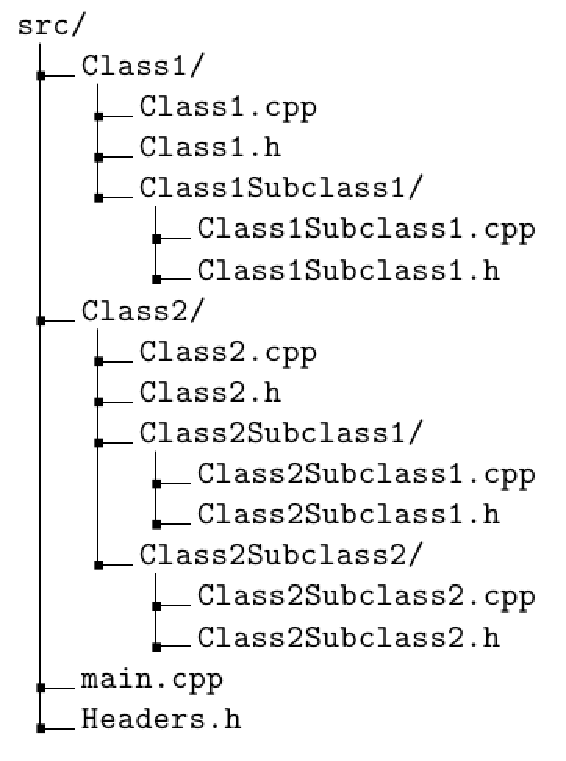
\includegraphics[scale=0.6]{../Graphics/SRCfolderStruct.pdf} 
 \end{center}

 \caption{An illustration of a standard way to organize source code. The file endings represent C++ code.}
 \label{FIG:SRCdirTree}
\end{figure}


\subsection{Class Structures}

In scientific programming, we are often in a situation where the simulated process has a physical - or mathematical interpretation. Examples are e.g. particles in molecular dynamics, atoms in bose-einstein condensates, random walkers in diffusion processes, etc. Choosing to create classes representing these quantities will shorten the gap between the mathematical formulation of the problem and the implementation.

In addition we have estimates such as energy, entropy and temperature, all of which are calculated based on equations from statisical mechanics or similar. Having class methods representing these calculations will again shorten the gap. There is no question what is done when the \verb+system.get_potential_energy+ method is called, however, if some random loop appears in the main solver, an initial investigation is required in order to understand the flow of the code.

As described in Section \ref{sec:typeCastPoly}, abstracting e.g. the potential energy function into a system object opens up the possibility of generalizing the code to any potential without altering the main solver. Structure is in other words vital if readability and versatility is desired. 

Planning the code structure comes in as a key part of any large coding project. For details regarding the planning of the code used in this thesis, see Section \ref{sec:AssGoal}.
